

\documentclass[11pt]{article}

\title{ }

\usepackage[top=0.5in, bottom=0.5in, left=0.5in, right=0.5in]{geometry}
\usepackage{helvet}
\usepackage{url} % hypderref?
\usepackage{graphicx}
\graphicspath{{figures/}} % The figures are in a figures/ subdirectory.
\renewcommand{\familydefault}{\sfdefault}
\pagestyle{empty}
%\pagestyle{plain}

% Fancy page-width tables
\usepackage{tabularx}

% Use a package for framed boxes
\usepackage{mdframed}

\usepackage[T1]{fontenc}
\usepackage{amssymb}


\usepackage{setspace}
\usepackage{microtype}

\usepackage{amsfonts}
\usepackage{amsmath}

\usepackage{floatrow}

\usepackage[normalem]{ulem} % for nci.bst

\usepackage{sidecap}
\usepackage[abs]{overpic}
\usepackage{wrapfig}


\usepackage{hyperref}
\hypersetup{colorlinks=true, urlcolor=black, citecolor=black, linkcolor=black}

\usepackage[numbers,sort&compress]{natbib} %comment on first run?

% \usepackage{multibib}
% %\newcites{full,sampl}{A,B}
% \newcites{sampl}{Full List of SAMPL References}
% %\newbibliography{full}

%\usepackage[round,authoryear]{natbib}
%\usepackage{cite}
%\setlength{\bibsep}{0.00in}


\newcommand{\doi}[1]{\href{http://dx.doi.org/#1}{doi:#1}}

\newcommand{\ac}[1]{{\sc \lowercase{#1}}}

\renewcommand{\baselinestretch}{.93}
%\renewcommand{\baselinestretch}{.90}
\usepackage{wrapfig}

% \usepackage{bibspacing}
% \setlength{\bibspacing}{\baselineskip}




\graphicspath{{figs/}}

\makeatletter

\newcommand{\captionfonts}{\footnotesize}

\makeatletter  % Allow the use of @ in command names
\long\def\@makecaption#1#2{%
  \vskip\abovecaptionskip
  \sbox\@tempboxa{{\captionfonts #1: #2}}%
  \ifdim \wd\@tempboxa >\hsize
    {\captionfonts #1. #2\par}
  \else
    \hbox to\hsize{\hfil\box\@tempboxa\hfil}%
  \fi
  \vskip\belowcaptionskip}
\makeatother

\renewcommand{\figurename}{{\bf Figure}}

% Page numbering.
%\pagestyle{plain}
%\pagenumbering{arabic}

\setlength{\abovecaptionskip}{-5pt}

\makeatother

\renewcommand{\refname}{Bibliography and References Cited}

\setlength{\parindent}{0pt} % Don't indent first line
%\setlength{\parskip}{1ex plus 0.5ex minus 0.2ex} % Add some space between paragraphs
\setlength{\parskip}{0.8ex} % Add some space between paragraphs

%%%%%%%%%%%%%%%%%%%%% c-bun's additions
\newcommand{\comment}[1]{\textit{\textcolor{red}{#1}}}
\usepackage{booktabs}
\usepackage{upgreek} % allows nonitalic greek letters
\usepackage{titlesec}
\titlespacing\subsubsection{0pt}{6pt plus 4pt minus 2pt}{0pt plus 2pt minus 2pt} % allows use of sections without all that extra spacing.
\renewcommand{\tablename}{{\bf Table}}
\includeonly{Authentication_of_Chemical_and_Biological_Resources}
%%%%%%%%%%%%%%%%%%%%% end c-bun's additions

\begin{document}

\documentclass[11pt]{article}
\usepackage[top=0.5in, bottom=0.5in, left=0.5in, right=0.5in]{geometry}
\usepackage{helvet}
\usepackage{url} % hypderref?
\usepackage{graphicx}
\graphicspath{{figures/}} % The figures are in a figures/ subdirectory.
\renewcommand{\familydefault}{\sfdefault}
\pagestyle{empty}
%\pagestyle{plain}

\usepackage{setspace}

\usepackage{amsfonts}
\usepackage{amsmath}

\usepackage{sidecap}
\usepackage[abs]{overpic}
\usepackage{wrapfig}

%\usepackage[round,authoryear]{natbib}
\usepackage{cite}
%\setlength{\bibsep}{0.00in}

\usepackage{hyperref}
\hypersetup{colorlinks=true, urlcolor=black, citecolor=black, linkcolor=black}

\newcommand{\doi}[1]{\href{http://dx.doi.org/#1}{doi:#1}}

\newcommand{\ac}[1]{{\sc \lowercase{#1}}}

\renewcommand{\baselinestretch}{.93}
%\renewcommand{\baselinestretch}{.90}
\usepackage{wrapfig} 

\usepackage{bibspacing}
\setlength{\bibspacing}{\baselineskip}


\graphicspath{{figs/}}

\makeatletter

\newcommand{\captionfonts}{\footnotesize}

\makeatletter  % Allow the use of @ in command names
\long\def\@makecaption#1#2{%
  \vskip\abovecaptionskip
  \sbox\@tempboxa{{\captionfonts #1: #2}}%
  \ifdim \wd\@tempboxa >\hsize
    {\captionfonts #1. #2\par}
  \else
    \hbox to\hsize{\hfil\box\@tempboxa\hfil}%
  \fi
  \vskip\belowcaptionskip}      
\makeatother

\renewcommand{\figurename}{Fig.}

% Page numbering.
%\pagestyle{plain}
%\pagenumbering{arabic}

\setlength{\abovecaptionskip}{-5pt}

\makeatother

\renewcommand{\refname}{Bibliography and References Cited}

\setlength{\parindent}{0pt} % Don't indent first line
\setlength{\parskip}{1ex plus 0.5ex minus 0.2ex} % Add some space between paragraphs

\begin{document}

%======================================

%%%%%%%%%%%%%%%%%%%%%%%%%%%%%%%%%%%%%%%%%%%%%%%%%%%%%%%%%%%%%%%%%%%%%%%%%%%
% HEADING
%%%%%%%%%%%%%%%%%%%%%%%%%%%%%%%%%%%%%%%%%%%%%%%%%%%%%%%%%%%%%%%%%%%%%%%%%%%

\begin{centering}
{\bf PROJECT NARRATIVE}

\end{centering}

% Using no more than two or three sentences, describe the relevance of this research training program to public health. In this section, use plain language that can be understood by a general, lay audience.
Physical methods for designing small molecule therapeutics are poised for a breakthrough, allowing molecular design for targeted treatment of diseases, personalized medicine, and rapid drug development. 
However, careful stress testing and improvement of these methods is necessary to make them sufficiently reliable and robust for the enormous range of problems they can potentially solve. 
Here, we will generate new experimental data on carefully selected and tailored systems, using it to drive a series of blind community challenges which follow a crowdsourcing model for testing and improving these methods, inducing new innovations and preparing the methods to have the dramatic impacts on human health that they promise. 

%======================================

%\setlength{\bibsep}{0.000in}

%\bibliographystyle{gec_nih}
%\bibliographystyle{ieeetr}
%\bibliographystyle{myrefstyle}
%\bibliography{chodera-research}


\end{document}







% !TEX root = ./Research_and_SA.tex

% FROM THE NIH SITE:
% Is the proposed research project of high scientific quality, and is it well integrated with the proposed research training plan?
% Based on the sponsor’s description of his/her active research program, is the applicant’s proposed research project sufficiently distinct from the sponsor’s funded research for the applicant’s career stage?
% Is the research project consistent with the applicant’s stage of research development?
% Is the proposed time frame feasible to accomplish the proposed training?

\noindent \begin{center}
{\bf SPECIFIC AIMS}
\end{center}

Genetically-encoded probes have revolutionized our understanding of cellular processes. Fluorescent proteins are a powerful technology that enable tracking of protein concentration and localization over large timescales and with single-molecule resolution. Via simple genetic manipulation, virtually any protein of interest can be labeled and tracked in the cell. However, analogous techniques for study of other biomolecules through genetic encoding (e.g. RNA)  are underdeveloped. There is currently no approach suitable for tracking the diverse types of RNAs found in mammalian cells. % Amy: suggested edit: "are far less developed and there is currently no approach suitable for tracking the diverse types of RNAs found in mammalian cells."

The importance of RNA in controlling a wide range of cellular functions has only recently been realized \cite{CechNoncodingRNARevolution2014}. Signaling by messenger and noncoding RNAs in the cell is highly dependent on the location of the transcripts. It is understood that cellular machinery modulates the location of these molecules, but these processes remain difficult to elucidate \cite{Muller-McNicollHowcellsget2013a}.
%Only (SOME FRACTION HERE) of RNA are actually involved in protein synthesis, while the rest is not well understood.
This lack of understanding is due in part to the lack of tools available to image this biomolecule. Localization of RNA on a single-molecule level, and multicomponent imaging of RNA transcripts remains difficult. Existing tools utilize aptamers that are unstable in mammalian cells \cite{EtzelSyntheticRiboswitchesPlug2017}, or constructs that are too large for imaging most transcripts. Multicomponent RNA imaging is also difficult due to the design of current tools.

To address this need, \textit{I aim to develop a platform for RNA imaging that will enable facile tracking of multiple transcripts at high resolution}. Riboglow is an RNA imaging platform recently developed in the Palmer lab. It utilizes a fluorescence-quenched pair formed by cobalamin (vitamin B\textsubscript{12}) and a pendant fluorophore. In solution, this construct shows low fluorescence. When bound to the cobalamin riboswitch aptamer domain \cite{JohnsonJrB12cofactorsdirectly2012}, there is an increase in fluorescence. This tool shows promise for RNA imaging because it solves many of the problems faced by traditional RNA probes.
The platform is similar to Spinach \cite{PaigeRNAMimicsGreen2011}, Broccoli \cite{FilonovBroccoliRapidSelection2014}, and Mango \cite{AutourFluorogenicRNAMango2018,DolgosheinaRNAMangoAptamerFluorophore2014} in that it utilizes a small molecule-binding aptamer for localization, but improves on these tools because it utilizes a natural aptamer that is more stable in the cellular environment (because of its native fold).
The current gold-standard for imaging is the MS2-FP system \cite{FuscoSinglemRNAMolecules2003}, which utilizes an stem-loop-binding bacteriophage coat protein fused to a fluorescent protein. Though this technique benefits from the modularity of fluorescent proteins, it requires large constructs to concentrate the fluorescent signal (24 stem-loops are often placed in series), thus precluding its use with most RNAs.

Riboglow is already a useful tool for RNA imaging, but several drawbacks are keeping it from widespread utility. The proposed work addresses these drawbacks, and seeks to utilize improved Riboglow tools to study outstanding questions in the field of noncoding RNA. The \underline{\textit{objective}} of the work is to image noncoding RNAs as they function within living cells. My \underline{\textit{central hypothesis}} is that the Riboglow platform can be improved through chemical modification and RNA selection to provide brighter, multicomponent probes.

{\bf \underline{Aim 1.} Synthesize improved Riboglow probes.}\\
Previously developed Riboglow constructs suffered from poor signal induction and low brightness. I aim to derivatize the native cobalamin structure to produce new probe scaffolds. The linker and fluorophore will also be varied with the goal to maximize fluorescence turn-on. These new molecules will be evaluated for quenching efficiency and will be tested with native cobalamin aptamers.

{\bf \underline{Aim 2.} Adapt Riboglow for single-molecule imaging.}\\
The molecules developed in \textit{Aim 1} will be screened against libraries of aptamers to further improve probe properties. Screening will be carried out in mammalian cells via flow cytometry. Candidate probes will be verified through imaging of mRNA transcripts in living cells.

{\bf \underline{Aim 3.} Develop mutually orthogonal Riboglow probes for multicomponent imaging.}\\
In tandem with brightness optimization, I will develop mutually orthogonal probes to enable labeling of different RNA transcripts in the same cell. The power of SELEX to find selective and tight binders will be used to screen for mutually exclusive aptamer-cobalamin pairs. These pairs will be conjugated to spectrally-resolved fluorophores to enable tracking of multiple RNA simultaneously. These orthogonal probes will be used to image long noncoding RNA and mRNA as they interact in the cell.

%%% Local Variables: ***
%%% mode: latex ***
%%% TeX-master: "Research_and_SA.tex" ***
%%% End: ***

% !TEX root = ./Research_and_SA.tex

\textbf{SIGNIFICANCE}
RNA lies at the center of cellular function. Its most appreciated function is to carry protein blueprints to the ribosome for manufacture. Only recently have researchers begun to appreciate its myriad of other functions, many of which also lie at the center of important cellular processes.\cite{CechNoncodingRNARevolution2014} \comment{X, Y, and Z (maybe the proposed test systems??)} have been recently found to have crucial RNA components.
\comment{Need more on these systems here. Talk about how localization is important.}
This importance for cellular function necessitates a toolset of probes to study these RNAs as they traverse the cell.
% TODO more here. look at RNA imaging paper intros for examples.

%%%%%%%%%%%%%%%%%%%%%%%%%%%%%%%%%%%%%%%%%%%%%%%%%%%%%%%%%%%%%%%%%%%%%%%%%%%%%%%%
%Riboglow
\begin{wrapfigure}[30]{r}{9cm}
%\vspace{-0.2in}
\begin{centering}
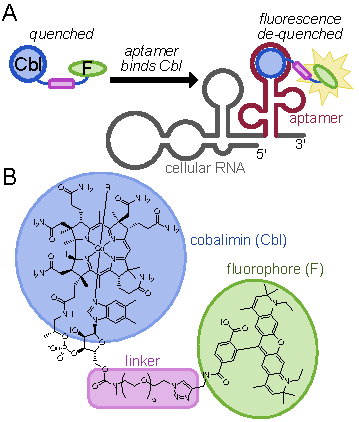
\includegraphics[width=\textwidth]{figures/fig1v2.pdf}

\end{centering}
\footnotesize
\caption{\label{figure:riboglow}
A) Cobalamin acts as a quenching and localization moiety to guide a fluorescent probe to an RNA transcript of interest. When unbound, fluorescence is quenched. In the presence of RNA tagged with the cobalamin aptamer, fluorescence is restored. B) Structure of the generation 1 Riboglow probe. A polyethylene glycol linker of five units (5xPEG) connected to the 5' hydroxly of the cobalamin ribose was used to tether an ATTO 590 fluorophore to the construct.
}
\end{wrapfigure}
%%%%%%%%%%%%%%%%%%%%%%%%%%%%%%%%%%%%%%%%%%%%%%%%%%%%%%%%%%%%%%%%%%%%%%%%%%%%%%%%

\textbf{BACKGROUND}
Protein studies benefit from a large imaging toolkit that has been developed over the last \comment{XX} years. Genetically encodable fluorescent proteins are now ubiquitous for the study of the localization of any translated target in the cell. While fluorescent proteins are a mature, well-understood technology, tools for imaging the localization of individual RNA transcripts remain limited. The most popular systems to date include dye-binding aptamers (Spinach\cite{PaigeRNAMimicsGreen2011}, Broccoli\cite{FilonovBroccoliRapidSelection2014}, and Mango\cite{AutourFluorogenicRNAMango2018,DolgosheinaRNAMangoAptamerFluorophore2014}), and RNA-binding protein fusions (MS2-FPs).\cite{FuscoSinglemRNAMolecules2003}

The most analogous to fluoresecent proteins, dye-binding aptamers utilize exogenously administered dyes that give fluorescence induction upon binding their RNA partner.\cite{PaigeRNAMimicsGreen2011,FilonovBroccoliRapidSelection2014,AutourFluorogenicRNAMango2018,DolgosheinaRNAMangoAptamerFluorophore2014} This sequence is encoded downstream of an RNA of interest to track its location in the cell. Though excellent binders for their dyes, the aptamers utilized by this technology are unstable in mammalian cells due to their nonnative structure.\cite{EtzelSyntheticRiboswitchesPlug2017} Additionally, though fluorescence turn-on is excellent \textit{in vitro}, signal induction in cells is low, most likely due to nonspecific binding of the dye.

RNA-binding protein fusions are a much more robust technique for imaging RNA transcripts.\cite{FuscoSinglemRNAMolecules2003} This method often utilizes the MS2 bacteriophage coat protein that binds an encoded stem loop of RNA. When MS2 is fused to a fluorescent protein, transcripts can be visualized in the cell. In order to concentrate the fluorescence signal above background, multiple stem loops are placed in series (up to 24 in a row). Though this technique has enabled imaging of single transcripts in the cell,\cite{MorisakiRealtimequantificationsingle2016,FuscoSinglemRNAMolecules2003} the resulting protein-RNA complex is prohibitively large for many studies.

\comment{Discuss RNA Fish here??}

Riboglow is a recently developed platform in the Palmer lab that solves many of the drawbacks of current RNA imaging techniques (Fig. \ref{figure:riboglow}). The two-component system utilizes a synthetic fluorophore-quencher pair, and a genetically-encoded aptamer. When the construct binds the transcribed aptamer, the fluorophore is dequenched, giving fluorescent signal. Like the dye-binding aptamers, Riboglow utilizes a riboswitch receptor domain that natively binds vitamin B\textsubscript{12} (cobalamin, Cbl, Fig. \ref{figure:riboglow}B).\cite{JohnsonJrB12cofactorsdirectly2012} Conveniently, cobalamin is known to act as a fluorescence quencher for a variety of fluorophores.\cite{RosendahlSynthesisbiologicalactivity1982,LeeDesignSynthesisCharacterization2009,SmeltzerSynthesisCharacterizationFluorescent2001} The cobalamin center is conjugated to the fluorophore through a flexible linker that promotes quenching in the unbound state, but enables the fluorophore to reside at a distance in the bound state (Fig. \ref{figure:riboglow}B).

The Palmer lab found that this initial generation of Riboglow has the potential to outperform the existing tools in the field. Its use of a naturally occurring riboswitch imparts stability to the construct that is not present in other aptamer-based techniques. Additionally, the use of a donor-quencher pair reduces nonspecific fluorescence in the unbound state. Such signal induction is low in the aptamer-binding dyes, and cannot be obtained at all with the MS2-fluorescent protein fusions. Due to these advantages, Riboglow outperformed Broccoli and the MS2 system in initial studies of stress granule (SG) detection in mammalian cells.

Though promising, the initial iteration of Riboglow has significant room for improvement. With initial constructs, signal induction upon aptamer binding never exceeded seven fold. Additionally, to effectively detect stress granules, four aptamers had to be placed in series to concentrate fluorescence signal. This high background precluded single-molecule imaging. Finally, the strategy cannot currently be used to monitor the location of multiple transcripts in tandem. Herein, I will propose strategies to overcome these limitations through simultaneous modulation of the small molecule construct and aptamer sequence. This is an undertaking for which I am uniquely suited, due to my experience of tandem modification of small molecule-protein interactions during my graduate studies. First, I will synthesize a variety of new Riboglow probes to optimize fluorescence quenching (Aim 1). Next, I will turn to the sequence of the aptamer itself. I'll design a screen for brightness that will select the best aptamer sequence to match the optimized probe structure (Aim 2). This new, brighter pair will be tested for single-molecule detection. Finally, I will use SELEX to identify mutually orthogonal probe-aptamer pairs for multicomponent RNA imaging (Aim 3).

\textbf{APPROACH \underline{Aim 1.} Synthesize improved Riboglow probes.}\\
The main drawback of Riboglow is the poor turn-on that is observed upon probe binding. In this aim, I intend to leverage my background in synthetic chemistry to produce a panel of diverse probe structures that improve fluorescence quenching (and thus signal induction). In previous studies in collaboration with Professor Dorota Gryko (see Gryko letter of support) a small number of linkers and fluorophores were evaluated for quenching and fluorescence turn-on. Linker length and fluorophore wavelength were varied to gauge the quenching ability of cobalamin. Remarkably some degree of quenching occurred in all of the constructs synthesized, regardless of the spectral overlap of the fluorophore and the cobalamin. \textit{To optimize probe function, I will vary linker composition, attachment point, and pendant fluorophore.}

%%%%%%%%%%%%%%%%%%%%%%%%%%%%%%%%%%%%%%%%%%%%%%%%%%%%%%%%%%%%%%%%%%%%%%%%%%%%%%%%
%Aim 1
\begin{wrapfigure}[25]{l}{10cm}
%\vspace{-0.2in}
\begin{centering}
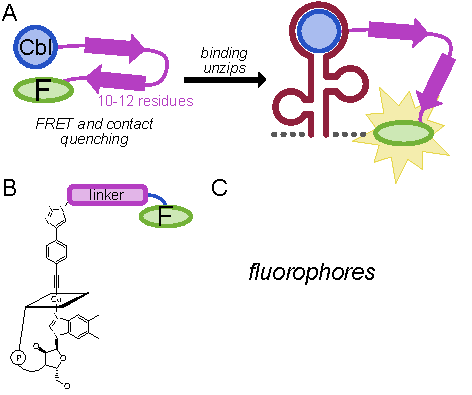
\includegraphics[width=\textwidth]{figures/aim1v2.pdf}

\end{centering}
\footnotesize
\caption{\label{figure:aim1}
A) Linkers. B) Conjugation sites. C) Fluorophores.
}
\end{wrapfigure}
%%%%%%%%%%%%%%%%%%%%%%%%%%%%%%%%%%%%%%%%%%%%%%%%%%%%%%%%%%%%%%%%%%%%%%%%%%%%%%%%

Ideally, in the unbound state, the cobalamin and fluorophore would be closely associated to maximize FRET and contact quenching.\cite{LeeDesignSynthesisCharacterization2009} In the RNA-bound state, the molecules would reside at their maximal distance to promote fluorescence. To strike this balance, I propose the use of a synthetic beta turn as the linker between cobalamin and the fluorophore (Fig. \ref{figure:aim1}A). Such a linker would hold the molecules close in solution, but would be linearized upon binding to the aptamer. A number of such beta turns have been developed. These motifs are as small as twelve amino acids and many are stable to denaturation up to 85 C.\cite{KierProbingLowerSize2008} In the unbound state, such a linker would hold the quencher and fluorophore in close proximity (due to the short distance between the N and C termini of the peptide). When the cobalamin is bound by an aptamer, steric occlusion would force the beta turn to unfold to place the fluorophore-quencher pair at a larger distance. The amino acids of the peptide linker will be varied to adjust the stability of the fold. \comment{More or less specific here? Discuss other linker possibilities?} The new constructs will be tested for their ability to quench fluorescence, and their fluorescence signal induction in the presence of the Riboglow aptamer.

Another underexplored variable of the original Riboglow probes is the linker attachment point. Though the 5' hydroxyl of the cobalamin ribose is the most accessible nucleophile on the structure, there exist several other possible sites of conjugation. Perhaps the second most common site is the axial ligand of the cobalt metal itself. Though many studies have taken advantage of the labile nature of certain alkyl modifications at this position,\cite{ShellVitaminB12Tunable2015} others have found alkynyl modifications to be stable to air and light.\cite{ChrominskiReductionfreesynthesisstable2013,RuetzMarkusPhenylethynylcobalaminLightStable2013} Following this precedent, I will synthesize a cobalamin with an alkyne handle attached to the cobalt metal center (Fig. \ref{figure:aim1}B). Such a molecule has already been synthesized in the lab of Dorota Gryko (see Gryko letter of support), and shown to be amenable to functionalization via dipolar azide-alkyne cycloaddition (AAC).\cite{ChrominskiVitaminB12Derivatives2014} The alkyne handle will be readily conjugated to a variety of linkers with terminal azides. \comment{More detail here?} These constructs will be evaluated for brightness in the presence and absence of the cobalamin aptamer.

%Fluorescence turn-on will also be modulated through changes to the cobalamin metal center. Changes to the electronic environment of the metal center will shift the absorption spectrum, enabling greater spectral overlap with the fluorophore to be quenched.\comment{[Cite]} As the \textit{de novo} synthesis of a molecule such as vitamin B12 would be a massive undertaking,\comment{[Cite]} I will target modifications that can be made through derivatization of the native structure. Without modification of the native ligand, variation of the axial position of cobalamin, and of the metal center itself should be straightforward. There is a large body of work that targets such modifications for the synthesis of so called ``antivitamins".\cite{KrautlerBernhardAntivitaminsB12Structure2015,ChrominskiReductionfreesynthesisstable2013} Through this undertaking, I will be in contact with Professor Dorota Gryko (see Gryko letter of support) one of the experts in this field.

The final variable in the molecular structure of the Riboglow probe is the fluorophore itself. The ideal probe would minimize cellular autofluorescence through the use of a red fluorophore with a high extinction coefficient. I believe that the Janelia Fluor series of dyes is perfectly suited for our application (see Lavis support letter).\cite{Grimmgeneralmethodfinetune2017a} \comment{Not sure how much else is needed here.}
%Previous work showed that probes were quenched by the cobalamin center to varying degrees. Quenching correlated somewhat with the spectral overlap of the fluorophore and cobalamin absorption.
% TODO is this 100% true? compare Cy5 excitation/emission with ATTO probes.
% TODO make a point here about how redder is better

\comment{Summary and alternate approaches here.}

\textbf{\underline{Aim 2.} Adapt Riboglow for superresolution imaging.}\\
Visualization of the lifecycle of single RNA transcripts as they move throughout the cell remains a holy grail of RNA imaging.\comment{[Cite]} Such a goal is possible via superresolution imaging and a probe with adequate photostability, and should be achievable with the Riboglow platform. With the wide variety of new probe constructs developed in Aim 1, changes will be made to the sequence of the cobalamin aptamer to increase fluorescence turn-on. A directed evolution screen for fluorescence brightness will identify optimal aptamer sequences that promote fluorescence signal induction.

%%%%%%%%%%%%%%%%%%%%%%%%%%%%%%%%%%%%%%%%%%%%%%%%%%%%%%%%%%%%%%%%%%%%%%%%%%%%%%%%
%Aim 2
\begin{wrapfigure}[25]{r}{10cm}
%\vspace{-0.2in}
\begin{centering}
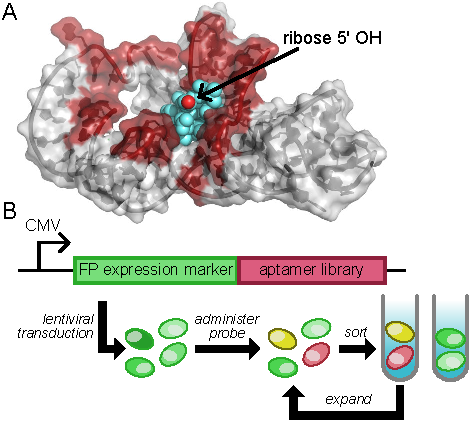
\includegraphics[width=\textwidth]{figures/aim2.pdf}

\end{centering}
\footnotesize
\caption{\label{figure:aim2}
A) Riboswitch sites for mutation will be targeted based on potential contact with the linker and fluorophore. PDB: 4FRN\cite{JohnsonJrB12cofactorsdirectly2012} B) RNA sequences will be screened for brightness relative to a fluorescent protein control.
}
\end{wrapfigure}
%%%%%%%%%%%%%%%%%%%%%%%%%%%%%%%%%%%%%%%%%%%%%%%%%%%%%%%%%%%%%%%%%%%%%%%%%%%%%%%%

First, a library will be designed that varies the environment surrounding the binding pocket of the cobalamin aptamer (Fig. \ref{figure:aim2}A). Though the guidance of Robert Batey (see Batey support letter), sites will be chosen to retain binding of the cobalamin, yet maximize the distance between the quencher and the fluorophore upon binding.\cite{JohnsonJrB12cofactorsdirectly2012} The Palmer lab is a leader in technologies for tool development in mammalian cells.\cite{FiedlerDropletMicrofluidicFlow2017,DeanHighSpeedMultiparameterPhotophysical2015} This expertise will be leveraged for screening libraries of cobalamin aptamers (Fig. \ref{figure:aim2}B). Libraries of transcripts will be transduced into mammalian cells, the probe of interest will be administered, and cells will be sorted via flow cytometry. Cells that show elevated brightness relative to a fluorescent protein expression control will be sequestered.
% QUESTION what is the absorption of Cbl bound to the riboswitch? does the spectrum change? Could we select for that?
In this way, libraries of up to one million members will be screened. Bright variants will be collected, cultured, and resubjected to sorting until only bright variants remain. Sequences will be evaluated through deep sequencing.

Candidate probes found through cell sorting will be verified in single molecule imaging experiments...

\comment{Summary and alternate approaches here.}

%%%%%%%%%%%%%%%%%%%%%%%%%%%%%%%%%%%%%%%%%%%%%%%%%%%%%%%%%%%%%%%%%%%%%%%%%%%%%%%%
%Aim 3: Multicomponent imaging
\begin{wrapfigure}[25]{l}{10cm}
%\vspace{-0.2in}
\begin{centering}
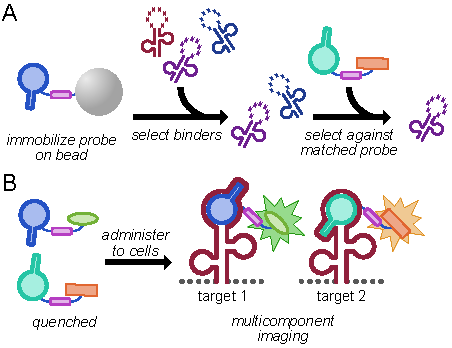
\includegraphics[width=\textwidth]{figures/aim3.pdf}
\end{centering}
\footnotesize
\caption{\label{figure:aim3}
A) SELEX will be used to screen for aptamers that bind each cobalamin in a mutually-exclusive manner. B) Mutually orthogonal cobalamin analogs will enable multicomponent RNA imaging. Signal turn-on will only be observed in the presence of the matched pair.
}
\end{wrapfigure}
%%%%%%%%%%%%%%%%%%%%%%%%%%%%%%%%%%%%%%%%%%%%%%%%%%%%%%%%%%%%%%%%%%%%%%%%%%%%%%%%

\textbf{\underline{Aim 3.} Develop mutually orthogonal Riboglow probes for multicomponent imaging.}\\
\comment{Don't forget Szostak precedent!\cite{LorschvitroselectionRNA1994}}
% TODO make a point here about how unnatural ligand architectures will help reduce off-target fluorescence.

%%% Local Variables: ***
%%% mode: latex ***
%%% TeX-master: "Research_and_SA.tex" ***
%%% End: ***

% !TEX root = ./Research_and_SA.tex

% FROM THE SITE:
% the reviewers will evaluate the adequacy of the proposed RCR training in relation to the following five required components:
% 1) Format - the required format of instruction, i.e., face-to-face lectures, coursework, and/or real-time discussion groups (a plan with only on-line instruction is not acceptable);
% 2) Subject Matter - the breadth of subject matter, e.g., conflict of interest, authorship, data management, human subjects and animal use, laboratory safety, research misconduct, research ethics;
% 3) Faculty Participation - the role of the sponsor(s) and other faculty involvement in the fellow’s instruction;
% 4) Duration of Instruction - the number of contact hours of instruction (at least eight contact hours are required); and
% 5) Frequency of Instruction – instruction must occur during each career stage and at least once every four years.

\begin{centering}
{\bf RESPONSIBLE CONDUCT OF RESEARCH}
\end{centering}

% TODO some stuff here about previous training and experience at UCI.

\begin{enumerate}
  \item{\bf Format}

  On a weekly basis the class will meet to hear a lecture from a member of the CU Boulder research faculty on a relevant topic on conduct of research. Immediately following each lecture, the class will break into small groups for discussion. Between classes, there will be assigned readings with accompanying questions to facilitate class discussion. Over the course of the semester, two case study essays will be written, reporting on real issues that researchers faced regarding one of the topics in the course.
  \item{\bf Subject Matter}

  The class reading will be from ``Responsible Conduct of Research'' by Adil Shamoo and David Resnik. (3rd ed. 2015, Oxford University Press)
  Topics will include: Why does RCR matter? The Scientist in Society. Mentor/Trainee Issues. Data Acquisition, Management, and Reproducibility. Lab Safety. Authorship, Publication, and Peer Review. Conflict of Interest. Research Misconduct. Protection of Human Subjects. Collaborative Research. Intellectual Property.
  \item{\bf Faculty Participation}

  In addition to interactions with faculty speakers during class, I will also meet with Professor Palmer on a biweekly basis to discuss responsible conduct of research during my first semester in the lab (Fall 2018). These meetings will cover data acquisition and storage, mentoring of graduate and undergraduate students, authorship, and collaboration in the Palmer lab. The lab also conducts monthly meetings on special research topics including
  \item{\bf Duration of Instruction}

  The class will meet on a weekly basis during the spring semester of 2019 for 15 weeks. Each class is two hours, giving a total of 30 contact hours.
  \item{\bf Frequency of Instruction}

  I will begin my postdoctoral studies in the fall of 2018, and enroll in the Responsible Conduct of Research class to be offered in the spring of 2019. This will fulfill the requirement for training during my postdoctoral career.
\end{enumerate}

%%% Local Variables: ***
%%% mode: latex ***
%%% TeX-master: "Research_and_SA.tex" ***
%%% End: ***

% !TEX root = ./Research_and_SA.tex

% FROM THE SITE:
% Are the sponsor(s’) research qualifications (including recent publications) and track record of mentoring individuals at a similar stage appropriate for the needs of the applicant?
% Is there evidence of a match between the research and clinical interests (if applicable) of the applicant and the sponsor(s)?
% If a team of sponsors is proposed, is the team structure well justified for the mentored training plan, and are the roles of the individual members appropriate and clearly defined?
% Are the research facilities, resources (e.g., equipment, laboratory space, computer time, subject populations), and training opportunities (e.g. seminars, workshops, professional development opportunities) adequate and appropriate?
% Is the institutional environment for the applicant’s scientific development of high quality?
% Is there appropriate institutional commitment to fostering the applicant’s mentored training.

\begin{center}
{\bf SELECTION OF SPONSOR AND INSTITUTION}
\end{center}

The proposed research will be carried out in the lab of Professor Amy Palmer in the Biofrontiers Institute at the University of Colorado Boulder. The Biofrontiers Institute is a world leader in both imaging and RNA research. In choosing this community to carry out my research, I am in an excellent position to be successful. RNA is a large focus of the institute. With Nobel Prize winner Tom Cech and its director, and the Rinn and Batey labs (see letters of mentoring support) in the same building, I will have easy access to the top researchers in the field of RNA. Collaboration with these labs will provide me with additional techniques and input that may not be readily available in the Palmer lab itself. The institute also provides superior research facilities and instrumentation that are maintained by full-time staff. Within the same wing as the Palmer lab is located both the cell culture facilities, and the microscopy core, and the building houses the deep sequencing and mass spectrometry cores.

I will also have a high chance of success due to my choice in mentor. Professor Palmer was educated by some of the best in the field, with her graduate degree in the lab of Edward Solomon at Stanford, and her postdoctoral work with Roger Tsien at the University of California, San Diego. She is an expert in the field of fluorescent tools development, and the study of fundamental cellular processes. When she was a postdoc in the Tsien lab, she was also awarded the Ruth L. Kirschstein National Research Service Award Postdoctoral Fellowship, thus she is aware of the level of training and mentorship that is necessary for awardees. Because my independent research goals lie in tool development at the interface of molecular organic chemistry and chemical biology, she is an excellent choice for training in this area. Additionally, professor Palmer has already mentored four group members that have gone on to acquire tenure-track professorships at research institutions.

%%% Local Variables: ***
%%% mode: latex ***
%%% TeX-master: "Research_and_SA.tex" ***
%%% End: ***

%!TEX TS-program = xelatex
\documentclass{F32}

\begin{document}



\begin{center}
\bf FACILITIES AND OTHER RESOURCES
\end{center}
More than adequate facilities for conducting the proposed research are available in the sponsor's laboratory, and in other core facilities across the Colorado University Boulder campus. These facilities, in addition to the scientific environment at CU Boulder, are more than sufficient to ensure the success of the proposed research. \textit{Major equipment in the sponsor's laboratory is described in the Equipment form.}

  {\bf The Jennie Smoly Caruthers Biotechnology Building (JSCBB):} Dr. Palmer’s laboratory is located in the new state-of-the-art Jennie Smoly Caruthers Biotechnology Building (JSCBB). JSCBB is a four-story, 330,000 square foot research building that houses more than 60 faculty members from the BioFrontiers Institute, the Department of Chemical and Biological Engineering, and the Division of Biochemistry. The building contains most of the core facilities that are crucial to the proposed research, in addition to the labs of professors Rinn and Batey, who will be offering mentoring support (see support letters).

  {\bf The Palmer Laboratory:} The Palmer lab is located on the third floor of JSCBB and covers approximately 3,000 feet of lab space shared with the Liu Lab. The lab occupies 5 research bays, each with 3--4 benches and 3 desk spaces. Located directly across the hall is \textit{(i)} the cell culture core facility, with all necessary equipment for mammalian cell culture, and \textit{(ii)} the imaging core facility that houses a variety of state-of-the-art microscopes. A cold room, autoclave and dishwashing room, dark rooms, and shared instrument rooms are located near the lab in JSCBB as well.

  {\bf BSL-2 Certified Cell Culture Core Facility:} Located directly across the hall from the Palmer lab is a fully-equipped mammalian cell culture facility with 12 biosafety cabinets, 24 double door incubators, automated liquid nitrogen storage units, and appropriate equipment (centrifuges, light microscopes, etc). The facility is BL-2 plus certified, enabling work with viruses and pathogens. The facility is staffed by Theresa Nahreini, who provides training and support.

  {\bf BioFrontiers Advanced Light Microscopy Core:} Also located across the hall from the Palmer lab, the Advanced Light Microscopy Core houses a number of advanced microscopes: a Nikon A1R resonant laser scanning confocal microscope with perfect focus, full environment chamber for long term imaging, and equipped with TIRF; a Nikon spinning disc confocal microscope with seven laser lines, equipped with a fully enclosed environmental chamber; an Image Express high throughput high content microscope; and a Nikon N-STORM system for super-resolution (more details on specific microscope capabilities in Equipment statement). An image analysis station is available with software including MATLAB, Imaris, Nikon Elements, ImageJ/Fiji, ICY, Cell Profiler. The facility is staffed by core director Dr. Joe Dragavon, who offers  training and assisted imaging sessions. Professor Palmer is the faculty advisor.

  {\bf BioFrontiers Next-Generation Genomics Facility:} Located in JSCBB, this facility houses an Illumina HiSeq 2000 sequencer, two MiSeq sequencers and associated Illumina iCompute infrastructure for analysis of sequencing data. Staff members aid in library construction and assessment of sequencing quality.

  {\bf Biomolecular Mass Spectrometry and Proteomics:} Also located in JSCBB, this facility specializes in both macromolecular and small-molecule mass spectrometry. The facility houses a LTQ-Orbitrap, and Orbitrap Velos mass spectrometer with CID/HCD/ETD fragmentation capabilities, interfaced with a Waters NanoAcquity 2D-UPLC system. Other instruments include a LTQ-Orbitrap mass spectrometer with CID fragmentation capabilities (used for other proteomics), interfaced with a Waters NanoAcquity 2D-UPLC system, a Waters Synapt G2 QqTOF mass spectrometer with Waters Acquity UPLC system (mainly used for small molecule and hydrogen-deuterium exchange studies), a PerSeptive Voyager DE-STR MALDI-TOF mass spectrometer, and a AB 4000 QTrap Linear Ion Trap mass spectrometer with Eksigent 2D-LC nanoflow HPLC. For small molecule analysis, the facility offers accurate mass determinations and complex mixture analysis.

  {\bf NMR Spectroscopy Facility:} In JSCBB, a Bruker Avance-III NMR spectrometer operating at 400MHz for proton NMR is available for walk-up use. It is capable of one and two-dimensional NMR experiments on most NMR-active nucleii, and is equipped with a 60-slot autosampler. This instrument is complemented by a larger facility nearby on campus containing a similar 300MHz instrument, a 400MHz Varian INOVA 400, and a 500 MHz Varian INOVA 500.

  {\bf Cell Sorting Facility:} Located directly across the hall from the Palmer Lab, the cell sorting facility contains a FACSAria III (BD Biosciences), and a MoFlo cell sorter from Cytomation. The facility, and training for its use is available to all labs in the building.

  {\bf Computers:} Several computers and data storage servers are available in the Palmer lab. The Biochemistry division of the Chemistry department also offers DEC and SUN workstations, and Silicon Graphics terminals for molecular modeling.

  {\bf The JSCBB Shared Instruments Pool:} JSCBB also houses a shared instruments pool that provides access to a variety of analytical instruments necessary for biochemical studies. The facility contains EPR, CD, and fluorescence spectrometers, an isothermal titration calorimeter, and other instruments.

  {\bf Institutional Postdoctoral Support and Resources:} \textit{See document ``Institutional Environment and Commitment to Training'' document.}

\end{document}

%!TEX TS-program = xelatex
\documentclass{F32}

\begin{document}

\begin{center}
\bf EQUIPMENT
\end{center}

The Palmer lab has access to all of the equipment needed to perform the work proposed, most of which is present in the lab, the BioFrontiers Advanced Light Microscopy Core, and the Cell Culture Facility (both of which are across the hall from the lab).

\begin{itemize}
  \item Synthesis \begin{enumerate}
    \item 2 chemical fume hoods, 1 equipped with a vacuum line for airfree synthesis
    \item Mettler electronic analytical balances
    \item Rotary Evaporators
    \item LabAlliance high-performance liquid chromatography (HPLC) solvent delivery system equipped with a Rainin UV-1 detector (located in the lab of Zhongping Tan)
    \item Applied Biosystems Pioneer continuous flow peptide synthesizer (located in the lab of Zhongping Tan)
  \end{enumerate}
  \item Imaging \begin{enumerate}
    \item Nikon Ti-Eclipse Inverted Fluorescence Microscope with a iXon3 CCD camera (Andor) and a Dual view camera (DV2, Andor) for FRET imaging
    \item Nikon A1R Laser Scanning Confocal and TIRF Inverted Microscope with iXon X3 EMCCD
    \item Molecular Devices ImageXpress Micro XL System for high throughput-high content fluorescence microscopy
    \item Olympus IX-81 Inverted Microscope
    \item Nikon N-STORM and TIRF inverted microscopes for super-resolution microscopy with three cameras (2x Andor Ixon Ultra 897 EMCCD, 1x Hamamatsu ORCA Flash4.0 sCMOS)
    \item Nikon Spinning Disc Confocal Microscope
    \item An image analysis workstation with software: MatLab, Imaris, Nikon Elements, ImageJ/Fiji, ICY, and Cell Profiler
  \end{enumerate}
  \item Cell Culture \begin{enumerate}
    \item Biosafety cabinets for mammalian cell work
    \item BSL-2-certified biosafety cabinet for lentiviral work
    \item Centrifuge and ultracentrifuge
    \item CO\textsubscript{2} cell culture incubator
    \item Refrigerators and freezers (4, -20, and -80 $^\circ$C)
    \item Table top fluorescence microscope
    \item FACSAria III cell sorter (BD Biosciences)
  \end{enumerate}
  \item Molecular Cloning \begin{enumerate}
    \item Molecular biology-grade water system
    \item Cold room (4 $^\circ$C)
    \item Temperature-controlled incubating shakers
    \item Protein and DNA gel electrophoresis and Western blotting equipment
    \item heating blocks
    \item 37 $^\circ$C incubator
    \item PCR thermocyclers
  \end{enumerate}
\end{itemize}
See document ``Facilities \& Other Resources'' for shared equipment within the BioFrontiers Institute.


\end{document}

%!TEX TS-program = xelatex
\documentclass{F32}

\begin{document}


\begin{center}
{\bf INSTITUTIONAL ENVIRONMENT AND COMMITMENT TO TRAINING}
\end{center}

\begin{enumerate}
  \item \textbf{The University of Colorado Boulder:} University of Colorado Boulder is home to the Postdoctoral Association of Colorado. This group provides a regular mailing list of announcements for a wide variety of professional development and funding opportunities. They also organize regular events with a focus on career development, networking, social activities and advocacy. The Office of Postdoctoral Affairs is another avenue of support on campus for postdoctoral training and career development. They offer a number of services to CU postdocs such as networking events, seminars, and tutorials. Postdoctoral researchers are also welcome to attend events hosted by the graduate school at CU Boulder, including workshops, lectures, and networking events. Postdoctoral researchers are also invited to participate in an array of scientific communication forums, such as serving as speakers for Supergroup meetings and at the Biochemistry annual retreat.

  \item \textbf{The BioFrontiers Institute:} The scientific environment within CU Boulder and the BioFrontiers Institute is excellent. Professor Palmer is a part of both the Department of Chemistry and Biochemistry, and the BioFrontiers Institute, directed by Nobel Laureate Tom Cech. The institute has become a leading organization for RNA research, with both highly established faculty such as Robert Batey (see support letter), Roy Parker (HHMI Investigator), and Tom Cech, and newcomers like John Rinn who has recently moved from Harvard (see support letter). Not only are all these labs within the same building (JSCBB), they also meet regularly as supergroups to talk about current research, and to find opportunities to collaborate. The Palmer lab participates in the Biophysics, Signaling and Cellular Regulation, Chemical Biology, RNA, and Bioinformatics supergroups which meet bi-weekly.

  \item \textbf{The Palmer Lab:} Professor Palmer implements a lab structure that fosters an environment of collaboration and mentorship. She meets one-on-one with each student and postdoc every two weeks to discuss data, their research project, and career goals. Professor Palmer and I will also use these meeting times to \textit{(a)} discuss my future research program, \textit{(b)} grant writing and proposal construction, and \textit{(c)} mentoring opportunities and strategies.
  The Palmer lab also holds weekly group meetings in which members of the lab present their recent findings. Once a month the lab holds a special topics meeting to discuss important practical matters surrounding research. Topics include data storage and management, conduct of research, responsible image analysis, and manuscript writing.
  Within the lab itself, benches and desks are arranged together, with an abundance of shared workspace that promotes conversation and collaboration amongst labmembers.

  \item \textbf{Additional Individual Mentorship:} In addition to mentorship under Professor Palmer, I will meet regularly with professors Rinn and Batey (see letters of support) and attend both Rinn lab and Batey lab group meetings. Full Professor Batey has been a professor at CU Boulder for 15 years, and is an expert in riboswitch biology and engineering. His advise and mentorship will be instrumental for Aims 2 and 3 of my proposal. Full Professor Rinn only recently moved to CU Boulder from Harvard. He is an authority on long noncoding RNA, and will be instrumental in the experimental design regarding the use of our new tools for imaging these understudied RNAs. Taken together, professors Palmer, Batey, and Rinn form the ideal mentoring team for a postdoc that is seeking to advance to a tenure-track research professorship. Each will bring unique viewpoints and resources that will ensure my success if funded.

\end{enumerate}


\end{document}

% !TEX root = ./Research_and_SA.tex
\begin{center}
{\bf RESOURCE SHARING PLAN}
\end{center}

This work will generate new reagents and data that will be made freely available. Discoveries made as a result of this proposal will be published in peer-reviewed journals, presented at scientific conferences, and shared with other scientists and the community through open discussions. Information will only be withheld if it endangers chances of publication or communication to the community.

\subsubsection*{Chemical Characterization and Resources}
All original synthetic compounds and characterization obtained, including Riboglow probes and their associated NMR, UV/Vis, mass spectra, etc. will be stored in the Palmer lab indefinitely and will be distributed by the following plan:
\begin{itemize}
  \item Original and unprocessed spectra and chromatographs will be sent directly to requesting laboratories via email within 2 weeks of the original request.
  \item All processed spectra will be provided in the supporting information of published journal articles for continuous long term access.
  \item If available, small samples of material will be sent directly to requesting laboratories using standard express mailing services within 2 weeks of the original request.
\end{itemize}

\subsubsection*{DNA}
All original DNA reagents (including primers, plasmids, and libraries) will also be stored in the Palmer lab indefinitely and distributed by the following plan:
\begin{itemize}
  \item Genetic data, including high-throughput sequence reads will be submitted to the appropriate NIH-funded repositories including the NCBI BLAST database (https://blast.ncbi.nlm.nih.gov/Blast.cgi).
  \item Genetic constructs in the form of plasmids will be submitted to Addgene (www.addgene.org).
  \item DNA reagents will be will be sent directly to requesting laboratories using standard express mailing services within 2 weeks of the original request, so long as sufficient stocks remain available
\end{itemize}
I agree to deposit these resources into the appropriate repository as soon as possible but no later than within one year of the completion of the funded project period for the parent award or upon acceptance of the data for publication.

% AMY I am also attaching a resource sharing plan for a proposal I submitted back in 2013 so it's a little lame.  For resource sharing plans what I have seen is that sequences get deposited, constructs are shared with add gene, protocols are made available on websites and / or in detailed supplementary methods of publications, large datasets (RNAseq etc) are made available.  Chemical resources (such as probes you develop) are more challenging because it can be a substantial amount of work to synthesis.  I don't think there is an expectation to make available.  But, I think it would be reasonable to include a statement that you will make small aliquots of  compounds available to the community for test experiments.  Sequences of all riboswtiches will be published and constructs available from Addgene.

%%% Local Variables: ***
%%% mode: latex ***
%%% TeX-master: "Research_and_SA.tex" ***
%%% End: ***

% !TEX root = ./Research_and_SA.tex
\begin{center}
{\bf AUTHENTICATION OF CHEMICAL AND BIOLOGICAL RESOURCES}
\end{center}

This application makes use of a variety of biological and chemical reagents: established cultured cell lines, specialty chemicals and peptides, and plasmid DNA. The authenticity of these resources will be established according to NIH guidelines. Our efforts in each area are briefly described below.

\begin{enumerate}
  \item {\bf Cell lines:} Model mammalian cell lines will be used for the proposed studies. All cell lines will be obtained from ATCC and will be used for less than 12 passages. Cell lines will be tested for mycoplasma every 6 months.
  \item {\bf Specialty chemicals and peptides:} Chemical reagents will be obtained from common suppliers (Sigma Aldrich, etc.) that provide QC authentication.  The integrity of purchased chemicals will also be verified using common analytical techniques (NMR, mass spec, etc.)  All new small molecules produced during the proposed work will also be rigorously characterized (via NMR, mass spec, HPLC, etc.).  It should be noted that the PI has over 8 years of experience in small molecule synthesis and characterization.
  Peptides produced via solid-phase peptide synthesis will be confirmed using LCMS.
  \item {\bf Plasmids:} Plasmids used to produce protein conjugates will be obtained from commercial sources with sequencing validation (Addgene). Plasmids produced in-house will be sequenced to confirm the open reading frame.
\end{enumerate}

% AMY You will also need to include a plan for authentication of chemical and biological resources.  This statement doesn't influence your score but is important to use.  Here you basically say that all cell lines will be obtained from ATCC and will be used for less than 12 passages.  That cell lines will be tested for mycoplasma every 6 months. I'm not sure how to authenticate chemical resources - presumably using NMR and mass spec to validate the structure and assess purity?

%%% Local Variables: ***
%%% mode: latex ***
%%% TeX-master: "Research_and_SA.tex" ***
%%% End: ***


%%%%%%%%%%%%%%%%%%%%%%%%%%%%%%%%%%%%%%%%%%%%%%%%%%%%%%%%%%%%%%%%%%%%%%%%%%%%%%%%%%%%%%%%%%%%%%%%%%%%%%
% BIBLIOGRAPHY
%%%%%%%%%%%%%%%%%%%%%%%%%%%%%%%%%%%%%%%%%%%%%%%%%%%%%%%%%%%%%%%%%%%%%%%%%%%%%%%%%%%%%%%%%%%%%%%%%%%%%%

%%\eject

%\footnotesize
%\scriptsize
%\bibliographystyle{acm}
%%\bibliographystylesampl{nci}
\bibliographystyle{nci}
%\bibliographystyle{achemso}
%\bibliographystyle{nar}
%\bibliography{full}{sampl-r01}{BIBLIOGRAPHY AND REFERENCES CITED}
%\bibliography{sampl}{sampl-r01}{REFERENCES FROM PRIOR SAMPL CHALLENGES}

%%\bibliographysampl{sampl}
%%\eject
\bibliography{library}

\end{document}
